\section{Experimental Setup}
\par A $1 \; cm$ diameter carbon fiber tube, motor mounts and supports cutout
off a $1\, in$ thick sheet of plastic are assembled to form the support
structure upon which the BLDC motor is mounted (Figure~\ref{fig::exptSetup}). A
silicon strain gauge based force sensor, ATI-gamma-FT9809, is mounted on the
base of the structure such that the thrust direction of the propeller is aligned
with its $X-axis$. The acquisition rate is set to $250\,Hz$ which is found to be
greater than the Nyquist frequency for capturing noise and other disturbances.
The sensor is interfaced through LabView for data acquisition.

\par The motor-propeller system whose dynamics are to be identified consists of
DJI Phantom T-Motor version-3 of $920\,kv$, DJI-9450 self-tightening  composite
propeller and an AIR $20\,A,\; 600\,Hz$ ESC. The system is controlled using
NI-myRio-1900 embedded device which runs a real-time loop at $250\,Hz$. The input
to the system is measured in PWM duty cycles as ratio, $0$ corresponding to
$0\,\%$ duty cycle and $1$ corresponding to $100 \, \%$ duty cycle. The output
thrust force is measured in Newtons (N).

\par The thrust is not directly transmitted to the force sensor but through the
support structure. The non-collocated nature of the inputs and outputs results
in a non-minimum phase system for force transmission by the support structure
(Figure~\ref{fig::freq_struct}). Thus, the structure imposes limitations on the
frequency range of the signals that can be transmitted unaltered. From frequency
response  of the structure the maximum frequency of the
signal that is transmitted without attenuation is close to $314 \, rad/s
(\approx 50 \, Hz)$ which is found to be sufficiently high for capturing the low
frequency dynamics of the motor-propeller system.

\begin{figure}[H]
    \begin{minipage}{0.49\textwidth}
        \begin{figure}[H]
            \centering
            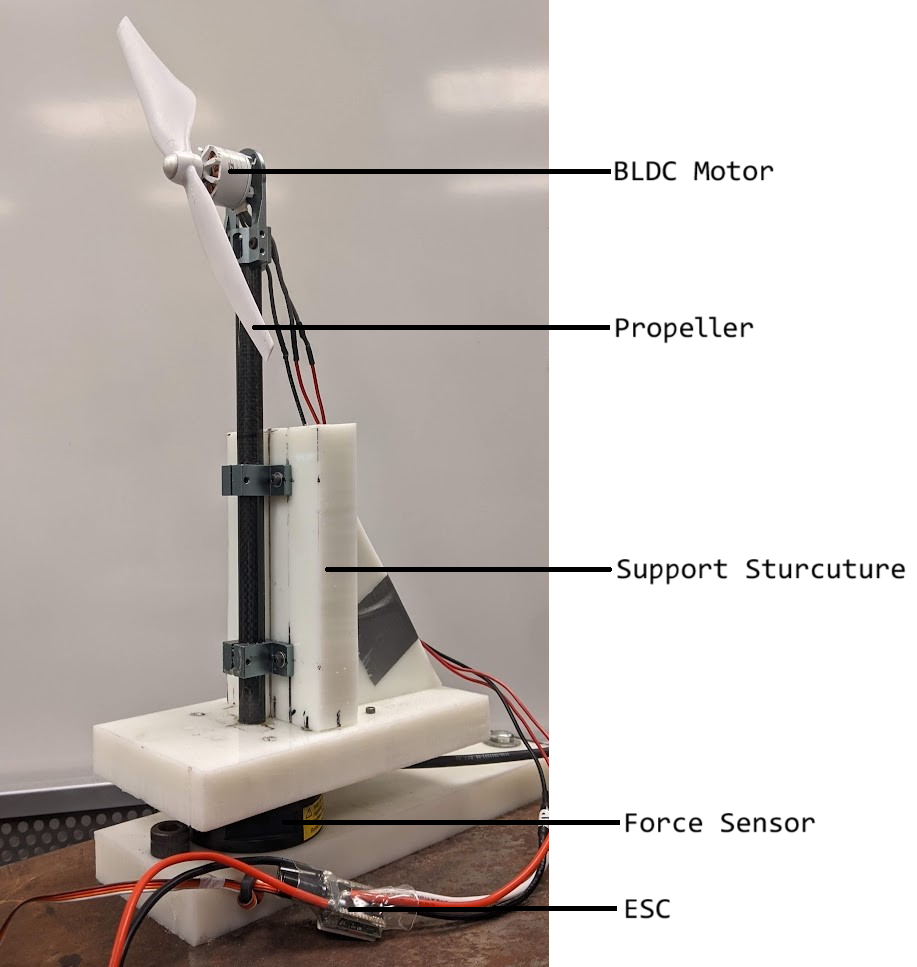
\includegraphics[height= 0.75\textwidth]{Part2/figs/2_figs/expt_setup/expt_setup.png}
            \caption{Experimental setup for system identification}
            \label{fig::exptSetup}
        \end{figure}
    \end{minipage}
    \begin{minipage}{0.49\textwidth}
        \begin{figure}[H]
                \centering
                \includegraphics[width = \textwidth]{Part2/figs/2_figs/expt_setup/struct_etfe.eps}
                \caption{Frequency response of the force transmission}
                \label{fig::freq_struct}
        \end{figure}
    \end{minipage}
\end{figure}
